\chapter{Global PID}
\label{chapter:globalpid}

\section{Introduction}
\label{pid_intro}

The global PID framework is designed to use sets of PID variables to 1) use MC data to create PDFs of these variables for a range of particle hypotheses, and 2) to use the PDFs as part of a log-likelihood method to determine the PID of reconstructed global tracks from data. The framework is designed such that new PID variables can be added as they are developed. Section 1 of this document will explain how to use the PID to produce PDFs, and how to perform PID on spill data contained within a Json document. Section 2 will detail how these two actions are performed within the code, and in Section 3 the PID variables, their structure, how new ones can be added to the framework, and details of those already in place, will be discussed. This document will be updated as the PID framework and variables continue to be developed.

\subsection{Using the PID scripts}
\label{pid_usage}

\subsection{Producing PDFs}
\label{pid_PDFs}
Whilst the PID framework will eventually come with PDFs provided (for the standard MICE beam settings) in  PIDhists.root, it is possible for a user to produce PDFs for hypotheses not included within this file. Due to current MC availability, users currently need to produce their own PDFs. The following describes how this should be done.
\begin{figure}[h!]
\begin{center} 
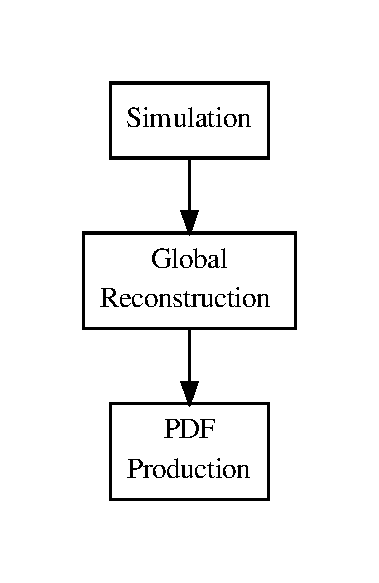
\includegraphics[width=2in]{reconstruction/globalpid/pdfprodflow.pdf} 
\caption{Steps invloved in producing a PDF from MC data}
\label{pdfprod}
\end{center} 
\end{figure}
\begin{itemize}
\item Simulation: Production of MC data for a given beam setting. Ideally G4Beamline input would be used, however input from spill generation in MAUS can be usedm but in the simulation datacards n\_particles\_per\_spill should be set to 1, as global track matching cannot process multiple particles per spill until there exists an MC trigger.
\item Global Track Reconstruction: The MC data should then be passed through 
the global track reconstruction, performed by MapCppGlobalReconImport and MapCppGlobalTrackMatching, which import the detector 
information into the global event and then construct the global tracks required 
for the calculation of PID variables. During the TrackMatching stage, it will have been possible for the user to choose to produce tracks for a single pid hypothesis or for several- for the purposes of PDF production a single hypothesis should be chosen, otherwise tracks will be duplicated. The choice of hypothesis doesn't matter as long as the track\_matching\_tolerances are set to large values (i.e. 10 x larger than those in ConfigurationDefaults.py). This is permissable as long as there is a single particle per spill in the simulation, as mentioned previously, because there will not be extra particles to be mis-matched to, and before the PDFs are populated the MC pid of the track is checked.
\item PDF Production: To produce the PDFs from the reconstructed MC 
data, pid\_pdf\_production.py in \$\{MAUS\_ROOT\_DIR\}\textbackslash 
bin\textbackslash Global is then used. This script calls the reducer 
ReduceCppGlobalPID. With this script, a datacard, such as that shown 
given in listing ~\ref{pdfdatacard}, that includes the datacards required to be set by the reducer, is used by entering at the command line:
\begin{verbatim}
> ${MAUS_ROOT_DIR}/bin/Global/pid_pdf_generator.py \
                    --configuration_file pdf_example_datacard.py
\end{verbatim}
This will create a directory within \$\{MAUS\_ROOT\_DIR\}\textbackslash files\textbackslash PID corresponding to the beam setting and identifier given by the datacard, which will then contain files for each PID variable, each of which will contain the PDF for each possible particle type. These can be combined into a single root file using the hadd command (see man pages for command usage).
\end{itemize}

\vspace*{1\baselineskip}

\begin{lstlisting}[language=Python,basicstyle=\ttfamily,frame=single,captionpos=b,caption={An example datacard (pdf\_example\_datacard.py) for use with pid\_pdf\_generator.py},label=pdfdatacard]
import os
import datetime

# Use the current time and date as a unique
# identifier when creating files to contain PDFs. 
# A unique_identifier is required by the reducer, 
# and PDF production will fail without one.
now = datetime.datetime.now()
unique_identifier = 
	now.strftime("%Y_%m_%dT%H_%M_%S_%f")

# A root file containing global tracks from MC
# data
input_json_file_name = 
	"global_track_input.root"

# PID MICE configuration, 'step_4' for Step IV running,
# 'commissioning' for field free commissioning data
# (straight tracks). Default is step_4
pid_config = "step_4"

# Tag used by both MapCppGlobalPID and
# ReduceCppGlobalPID, determines which PDFs to
# perform PID against/which PDFs to produce (in this
# case, set based upon input MC beam). A typical tag
# here would be the emittance and momentum, e.g.
# 3-140, 6-200, etc. Alternatively, users may choose to
# enter the run number they are simulating for here.
# The tag used for the PDFs must match the tag you
# use when doing PID
pid_beam_setting = "6-200"

# Polarity of running mode, value can be "positive"
# or "negative".
pid_beamline_polarity = "positive"

\end{lstlisting}


\vspace*{2\baselineskip}


\subsubsection{Performing PID with pre-existing hypotheses}
\label{pid_perf}
To perform PID on data, the steps shown figure ~\ref{pidperf} should be followed.

\begin{figure}[h!]
\begin{center} 
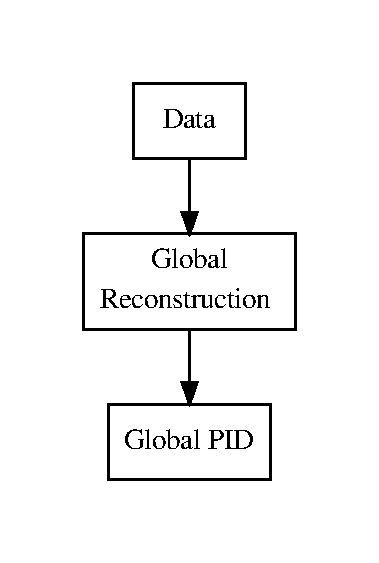
\includegraphics[width=2in]{reconstruction/globalpid/pidperfflow.pdf} 
\caption{Steps invloved in performing the PID for a data sample}
\label{pidperf}
\end{center} 
\end{figure}
			
\begin{itemize}
\item Data: This can be experimental or MC data.
\item Global Reconstruction: In the same way as described above for PDF generation, the 
data should then be passed through the global reconstruction.
\item Global PID: To perform the PID on the reconstructed data, GlobalPID.py in\linebreak\$\{MAUS\_ROOT\_DIR\}\textbackslash 
bin\textbackslash Global is then used. This script calls the 
MapCppGlobalPID mapper. With this script, a datacard, such as that 
shown given in listing ~\ref{piddatacard}, that includes the input and output root filenames, is used, by entering the following at the command line:
\begin{verbatim}
> ${MAUS_ROOT_DIR}/bin/Global/GlobalPID.py \
                    --configuration_file example_pid_datacard.py
\end{verbatim}
\end{itemize}

\begin{lstlisting}[language=Python,basicstyle=\ttfamily,breaklines=true,frame=single,captionpos=b,caption={An example datacard (example\_pid\_datacard.py) for use with GlobalPID.py},label=piddatacard]
import os

# A root document containing global tracks
input_root_file_name = 
	"global_recon_output.root"

# Output root file with track pid info included
output_root_file_name = 
	"output_Global_PID.root"

# Path to PDFs file. Users should enter the path
# to their own PDFs file here
PID_PDFs_file = " "

# PID MICE configuration, 'step_4' for StepIV running,
# 'commissioning' for field free commissioning data
# (straight tracks). Default is step_4
pid_config = "step_4"

# PID running mode - selects which PID variables are
# used. 'online' corresponds to less beam (momentum)
# dependent variables, 'offline' uses all variables 
# and requires that specific PDFs already exist for
# the beam.
pid_mode = "offline"

# Tag used by both MapCppGlobalPID and
# ReduceCppGlobalPID, determines which PDFs to
# perform PID against/which PDFs to produce (in this
# case, set based upon input MC beam). A typical tag
# here would be the emittance and momentum, e.g.
# 3-140, 6-200, etc. Alternatively, users may choose
# to enter the run number they are simulating for
# here. The tag used for the PDFs must match the tag
# you use when doing PID
pid_beam_setting = "6-200"

# Polarity of running mode, value can be "positive"
# or "negative".
pid_beamline_polarity = "positive"

# PID confidence level = set the margin (in percent)
# between the confidence levels of competing pid
# hypotheses before they are selected as the correct
# hypothesis
pid_confidence_level = 10

# PID track selection- select which tracks from
# TrackMatching to perform PID on. Can perform PID on
# all tracks by setting to "all", on through tracks
# only (constituent tracks will be PID'd, so this
# excludes orphans) with "through" or on all upstream
# and downstream tracks (ignoring whether tracks have
# been through-matched) with "constituents"
pid_track_selection = "all"

\end{lstlisting}

As the framework currently stands, the output file would now contain the global tracks with the PID set (where it has been possible to do so) to whichever particle hypothesis had the highest confidence (if it passes the confidence level cut), and the mapper name of the track will have been set to MapCppGlobalPID-<pid\_track\_selection>, e.g. if the datacard setting was pid\_track\_selection = "Through", the mapper name would be MapCppGlobalPID-Through.

\section{MapCppGlobalPID and ReduceCppGlobalPID}
\label{pid_mapred}
\subsection{MapCppGlobaPID}
\label{pid_map}
The steps taken in MapCppGlobalPID for a single track are shown in 
figure \ref{mapflow}. To express this more fully, the data, having passed through the global reconstruction, is then passed to the PID. For each track, the values of each PID variable are calculated. Each of these values is then compared to the corresponding PDFs for all particle hypotheses, the number of entries in the corresponding bin providing the probability from which the log-likelihood is calculated. For each particle hypothesis, the log-likelihoods of all of the PID variables are summed to give a log-likelihood for that hypothesis. The PID of the track is then obtained by comparing the log-likelihoods of the hypotheses.
\begin{figure}[h!]
\begin{center} 
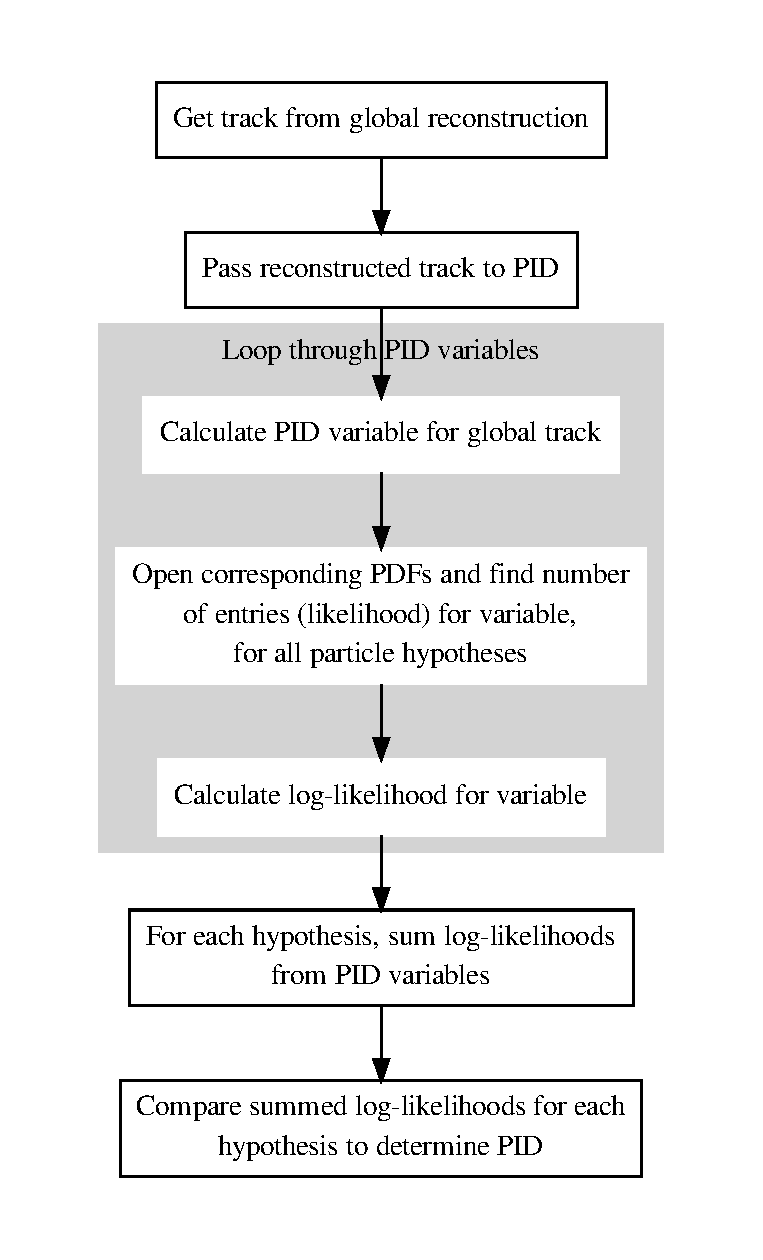
\includegraphics[width=3in]{reconstruction/globalpid/PIDflow.pdf} 
\caption{Flow chart detailing steps taken in MapCppGlobaPID}
\label{mapflow}
\end{center} 
\end{figure}

\section{ReduceCppGlobalPID}
\label{pid_reducer}
The steps taken in ReduceCppGlobalPID are shown in figure ~\ref{reduceflow}. MC data for a given particle hypothesis, having passed through the global reconstruction, is then passed to the PID. For each track, the values of each PID variable are calculated. A histogram is filled with these values. If the behaviour has been turned on in the PID variable class, then a single event is spread over all bins in the histogram, to ensure that when the PDF is used by the PID, there will no empty bins, thus avoiding cases where the log-likelihood takes the log of zero. The histogram is then normalised to create the PDF, which is then written and saved to file.
If a MC track returns a variable value outside of the allowed range of the histogram (as defined within the variable class) then the value for that track is not included.
\begin{figure}[h!]
\begin{center} 
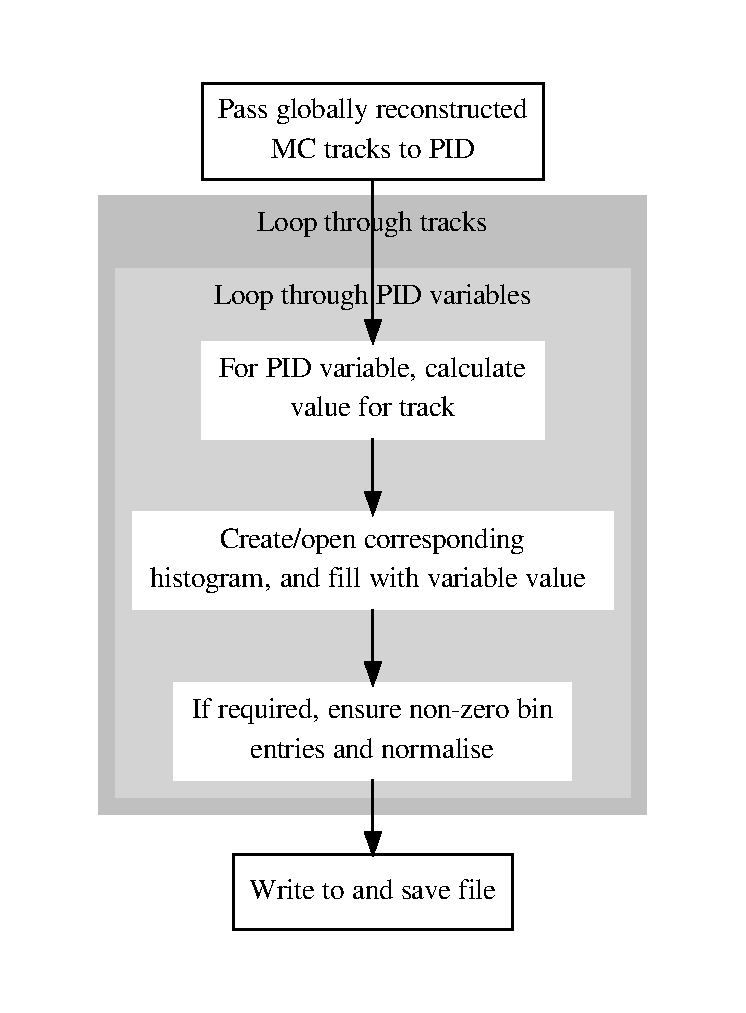
\includegraphics[width=3in]{reconstruction/globalpid/PDFflow.pdf} 
\caption{Flow chart detailing steps taken in ReduceCppGlobaPID}
\label{reduceflow}
\end{center} 
\end{figure}

\section{PID Variables}
\label{PID}
Information from the MICE detectors are incorporated into a set of 
PID variables that can be used to distinguish between particle 
hypotheses.
The Global PID framework has been written such that any number of PID 
variables can be developed and added as necessary, all represented by 
their own class, derived from a base class.

\subsection{PID Base Class}
\label{PIDBase}
The base PID class (PIDBase.hh and .cc) contains the functions to:
\begin{itemize}
\item Create the PDFs (and the files that contain them)
\item Use the PDFs with globally reconstructed tracks
\item Populate the PDFs with variable values (after checking that 
value is valid)
\item Perform the log-likelihood for an incoming globally reconstructed 
track (after checking that value of variable for track falls within 
range of PDF).
\item Calculate the value of the PID variable (this is a virtual 
function to be defined in the derived classes)
\end{itemize}

There are separate base classes for single value variables (PIDBase1D) and dual value variables (PIDBase2D).

\subsection{PID Variable Classes}
\label{PIDVar}
Each PID variable will be implemented in a derived class of the appropriate base PID class. Because of how the framework is designed, new variables can be added as they are developed. There are currently two sets of variables, those to be used when there is no field in the spectrometer solenoids (commissioning variables, ComPIDVars) and those to be used during Step IV running (PIDVars). 

\subsubsection{ComPIDVars}
\vspace {0.5cm}
\begin{tabular}{| l | l | p{5cm} |}
  \hline                       
  \textbf{PID} class & \textbf{Variable name}  & \textbf{Definition} \\\hline
  ComPIDVarA & diffTOF2TOF1 & Uses the time of flight between TOF1 and TOF2. Beam dependent. \\\hline
  ComPIDVarB & KLChargeProdvsDiffTOF1TOF2 & Uses the KL ADC charge product, and the time of flight between TOF1 and TOF2. \\\hline
  ComPIDVarC & CommissioningKLADCChargeProduct & Uses the KL ADC charge product . Beam dependent.\\\hline
  ComPIDVarD & CommissioningEMRrange &Uses the range of the particle as measured in the EMR. Beam dependent. \\\hline
  ComPIDVarE & CommissioningEMRrangevsDiffTOF1TOF2 & Uses the range of the particle as measured in the EMR, and the time of flight between TOF1 and TOF2.\\\hline
  ComPIDVarF & CommissioningEMRPlaneDensity & Uses the plane hit density in the EMR. Beam dependent.\\\hline
  ComPIDVarG & CommissioningEMRPlaneDensityvsDiffTOF1TOF2 & Uses the plane hit density in the EMR, and the time of flight between TOF1 and TOF2.\\\hline
  ComPIDVarH & CkovAvsDiffTOF1TOF2 & Uses the number of photoelectrons in Cherenkov A, and the time of flight between TOF1 and TOF2.\\\hline
  ComPIDVarI & CkovBvsDiffTOF1TOF2 & Uses the number of photoelectrons in Cherenkov B, and the time of flight between TOF1 and TOF2.\\
  \hline 
\end{tabular}

\vspace {0.5cm}


\subsubsection{PIDVars}

\vspace {0.5cm}
\begin{tabular}{| l | l | p{7cm} |}
  \hline                       
  \textbf{PID class} & \textbf{Variable name} & \textbf{Definition} \\\hline
  PIDVarA & diffTOF1TOF0 & Uses the upstream time of flight, between TOF0 and TOF1. This variable is beam dependent and so is best used during offline data analysis where PDFs can be produced for specific beam settings. \\\hline
  PIDVarB & diffTOF0TOF1vsTrackerMom & Uses upstream time of flight, and momentum as measured in the upstream Tracker. \\\hline
  PIDVarC & KLChargeProdvsDSTrackerMom & Uses the KL ADC charge product and the momentum measured in the downstream Tracker. \\\hline
  PIDVarD & KLADCChargeProduct & Uses the KL ADC charge product. This variable is beam dependent, and so is best used during offline data analysis.\\\hline
  PIDVarE & EMRRange & Uses the range of the particle as measured in the EMR. This variable is beam dependent, and so is best used during offline data analysis. \\\hline
  PIDVarF & EMRRangevsDSTrackerMom & Uses the range of the particle as measured in the EMR, and the momentum measured in the downstream Tracker. \\\hline
  PIDVarG & EMRPlaneDensity & Uses the plane hit density in the EMR. This variable is beam dependent, and so is best used during offline data analysis.\\\hline
  PIDVarH & EMRPlaneDensityvsDSTrackerMom & Uses the plane hit density in the EMR, and the momentum measured in the downstream Tracker.\\\hline
  PIDVarI & CkovAvsUSTrackerMom & Uses the number of photoelectrons in Cherenkov A, and the momentum measured in the upstream Tracker.\\\hline
  PIDVarJ & CkovBvsUSTrackerMom & Uses the number of photoelectrons in Cherenkov B, and the momentum measured in the upstream Tracker.\\
  \hline 
\end{tabular}

\subsubsection{Adding PID Variables}
\label{addvar}
In each derived variable class, the following should be included:
\begin{itemize}
\item The variable name should be set
\item The function to calculate the PID variable should be defined.  
\item If a valid value of a variable is not returned by the function, for instance due to missing measurements, then the value should be set to -1 so that it falls outside of the range of any PDFs.
\item The minimum, maximum, and number of bins for PDFs created using 
the variable should be set. The values of the minimum and maximum 
define the allowed range of values that the PID variable can take.
\item In some cases it may be necessary to ensure that all bins in a 
PDF return non zero entries, and so by setting the variable 
\_nonZeroHistEntries to true, a single event spread accross all bins 
will be added
\end{itemize}

\subsubsection{Placing cuts on PIDVar value ranges}
A further option for users when performing PID against the PDFs, is to cut on what range of values within the PDFs to perform PID within. This may allow for greater purity (potentially at the expense of efficiency) depending on the variable. For instance, one could choose to cut harshly on the time of flight in PIDVarA, to reduce the chances of mis-identifying pions as muons. These cuts can be selected through setting the appropriate pid\_bounds datacards found in ConfigurationDefaults.py.
